\documentclass[t]{beamer}

% --- Theme and Color Setup ---
\usetheme{Madrid}

% Define the custom Orange color
\definecolor{MyOrange}{RGB}{230, 85, 10} 

% Apply the orange color to the structure
\usecolortheme[named=MyOrange]{structure}

% Fix footer colors to match the orange theme
\setbeamercolor{palette primary}{bg=blue!90!black,fg=white}
\setbeamercolor{palette secondary}{bg=blue!70!black,fg=white}
\setbeamercolor{palette tertiary}{bg=blue!70!black,fg=white}
\setbeamerfont{caption}{size=\footnotesize}

% Packages
\usepackage[utf8]{inputenc}
\usepackage{hyperref}
\usepackage{tikz} 
\usepackage{booktabs}
\usepackage{natbib}

% --- 1. CONFIGURATION FOR CONTENT SLIDES (Middle Pages) ---
\addtobeamertemplate{frametitle}{}{%
    \begin{tikzpicture}[remember picture,overlay]
        \node[anchor=north east, xshift=-0.3cm, yshift=0cm, inner sep=0pt] at (current page.north east) {
            
\includegraphics[height=1cm, keepaspectratio]{logo1.png}
        };
    \end{tikzpicture}%
}

% --- 2. CONFIGURATION FOR FIRST & LAST PAGE ---
\newcommand{\FirstLastPageLayout}{
    \begin{tikzpicture}[remember picture,overlay]
        \node[anchor=north east, xshift=-0.3cm, yshift=0cm, inner sep=0pt] at (current page.north east) {
            
\includegraphics[height=1cm, keepaspectratio]{logo1.png}
        };
        \node[anchor=south west, xshift=0.5cm, yshift=0.5cm] at (current page.south west) {
            \textcolor{MyOrange}{\footnotesize Prague University of Economics and Business}
        };
    \end{tikzpicture}
}

% --- Info ---
\title[Title]{Title of your presentation} % 
\subtitle{Subtitle of your presentation} % 
\author{Your Name} % 
\institute[]{Department of International Economic Relations} % 
\date{\today}

\begin{document}

% --- Slide 1: Title Page ---
\begin{frame}
    \FirstLastPageLayout % 
    \titlepage
\end{frame}




% --- Research gap \& Aim of the paper ---
\begin{frame}{Research gap \& Aim} % 
    \begin{itemize}
        \item To insert a table...
    \end{itemize}
    \begin{table}[h!]
\centering
\caption{Summary statistics of XX} \label{HHI_table}
\begin{tabular}{lrrr}
\hline
Country & Mean X & Min X & Max X \\
\hline
AT & 0.29 & 0.28 & 0.30  \\
BE & 0.27 & 0.25 & 0.29 \\
BG & 0.23 & 0.20 & 0.28 \\
\hline
\multicolumn{4}{@{}l} {\tiny Source: own elaboration based on }
\end{tabular}
\end{table}
\end{frame}



% --- Methodology ---
\begin{frame}{Methodology} % 
    \begin{itemize}
        \item Your text
    \end{itemize}
\end{frame}



% --- Results \& Discussion ---
\begin{frame}{Results \& Discussion} % 
    \begin{itemize}
        \item To include a figure...
    \end{itemize}

    \begin{figure}
                \caption{XYZ}
             
                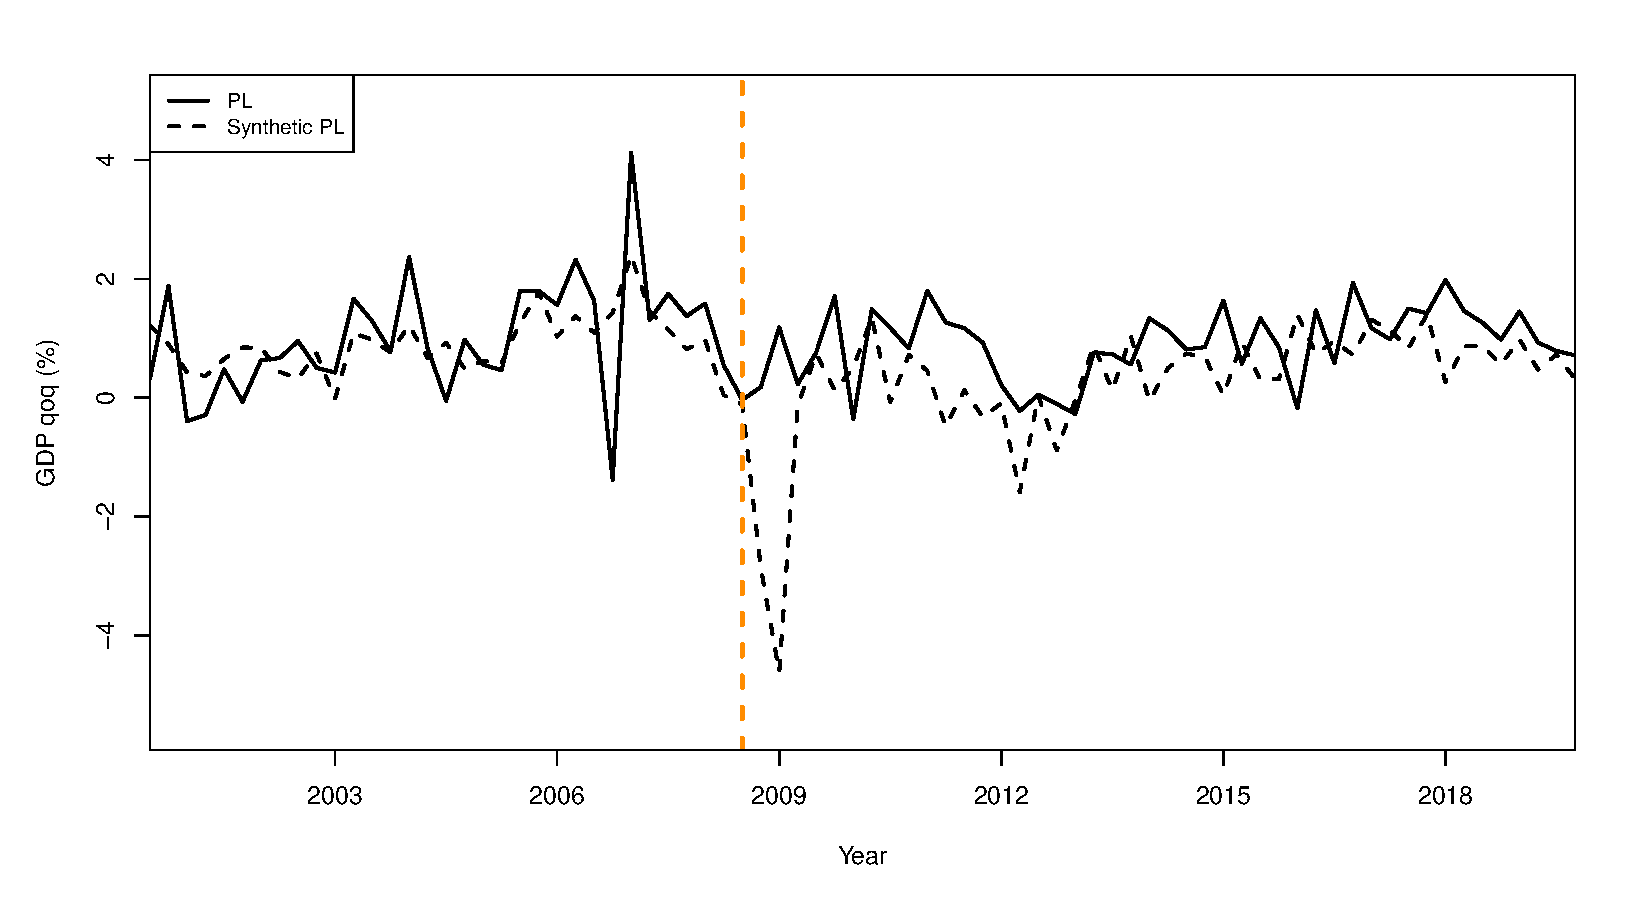
\includegraphics[width=7cm]{PL_GDP.pdf}
                
                {\tiny Source: Authors' calculations}
            \end{figure}

\end{frame}



\begin{frame}[allowframebreaks]{References}

\tiny
\bibliography{references}
\bibliographystyle{apalike}

\end{frame}



\end{document}